\documentclass[assignment = 2]{homework}

\usepackage{caption, subcaption, pdfpages, float}
\usepackage{graphics, wrapfig, pgf, graphicx}
\usepackage{enumitem}
\graphicspath{{../}}


% pacotes para importar código
\usepackage{caption, booktabs}
\usepackage[section, newfloat]{minted}
\definecolor{sepia}{RGB}{252,246,226}
\setminted{
    bgcolor = sepia,
    style   = pastie,
    frame   = leftline,
    autogobble,
    samepage,
    python3,
}
\setmintedinline{
    bgcolor={}
}

% ambientes de códigos de Python
\newmintedfile[pyinclude]{python}{}
\newmintinline[pyline]{python}{}
\newcommand{\pyref}[2]{\href{#1}{\texttt{#2}}}

% \SetupFloatingEnvironment{listing}{name=Código}
% \captionsetup[listing]{position=below,skip=-1pt}

\usepackage{csquotes}
\usepackage[style=verbose-ibid,autocite=footnote,notetype=foot+end,backend=biber]{biblatex}
\addbibresource{referencias.bib}
\usepackage[section]{placeins}

\usepackage[hidelinks]{hyperref}
\usepackage[noabbrev, nameinlink, brazilian]{cleveref}
\hypersetup{
    pdftitle  = {MC920 - Trabalho 2 - 187679},
    pdfauthor = {Tiago de Paula}
}

\newcommand{\textref}[2]{
    \hyperref[#2]{#1 \ref*{#2}}
}

\usepackage{import}
\usepackage{tikz}
\usetikzlibrary{matrix}
\usetikzlibrary{positioning}

\newenvironment{kmatrix}{
    \begin{tikzpicture}[node distance=0cm]
        \tikzset{square matrix/.style={
                matrix of nodes,
                column sep=-\pgflinewidth, row sep=-\pgflinewidth,
                nodes={draw,
                    minimum height=0.7cm,
                    anchor=center,
                    text width=0.7cm,
                    align=center,
                    inner sep=0pt
                },
            },
            square matrix/.default=0.7cm
        }
}{
    \end{tikzpicture}%
}

\newcommand*{\Scale}[2][4]{\scalebox{#1}{\ensuremath{#2}}}%

\newcommand{\red}[1]{\textcolor{red}{\textbf{#1}}}

\begin{document}

    \pagestyle{main}

    \section{Introdução}

Este trabalho teve como objetivo a implementação de técnicas de pontilhado com difusão de erros. A ideia é reduzir a quantidade de cores tentando manter a imagem o mais próximo possível da original. Isso é feito reduzindo a intesidade para seu limite mais próximo, ao longo de um caminho pela imagem, mas aplicando uma distribuição de erros na vizinhança do pixel.

A \cref{fig:base} apresenta as imagens base deste trabalho, usadas para análise e discussão das formas diferentes de aplicar o pontilhado. As figuras \ref{fig:baboon} e \ref{fig:peppers} são $512 \times 512$, enquanto a \cref{fig:monalisa} é $256 \times 256$ e a \cref{fig:watch} é $1024 \times 768$. Ao todo serão aplicadas 6 distribuições de erro com \red{2 curvas} diferentes. As distribuições de erros serão apresentadas ao longo do relatório, na \red{seção ??}, equanto as curvas podem ser encontradas na \red{seção ??}.

\begin{figure}[H]
    \centering
    \begin{subfigure}{0.33\textwidth}
    \centering
    \includegraphics[width=4.4cm]{imagens/baboon.png}
    \caption{\texttt{imagens/baboon.png}}
    \label{fig:baboon}
\end{subfigure}%
\begin{subfigure}{0.33\textwidth}
    \centering
    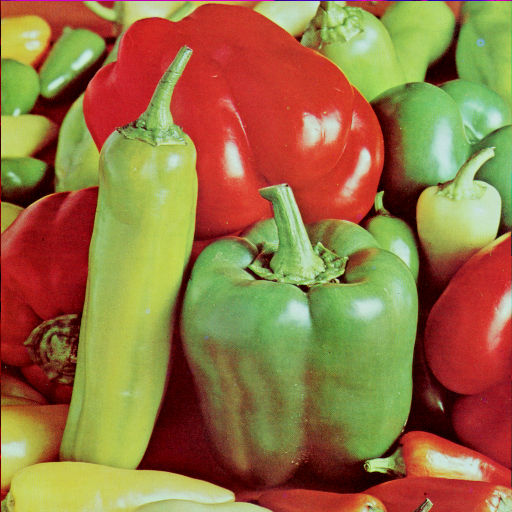
\includegraphics[width=4.4cm]{imagens/peppers.png}
    \caption{\texttt{imagens/peppers.png}}
    \label{fig:peppers}
\end{subfigure}\\[8pt]
\begin{subfigure}{0.33\textwidth}
    \centering
    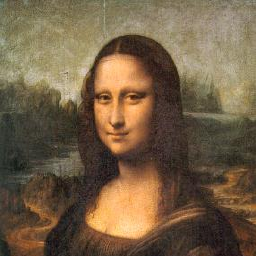
\includegraphics[width=4.4cm]{imagens/monalisa.png}
    \caption{\texttt{imagens/monalisa.png}}
    \label{fig:monalisa}
\end{subfigure}%
\begin{subfigure}{0.33\textwidth}
    \centering
    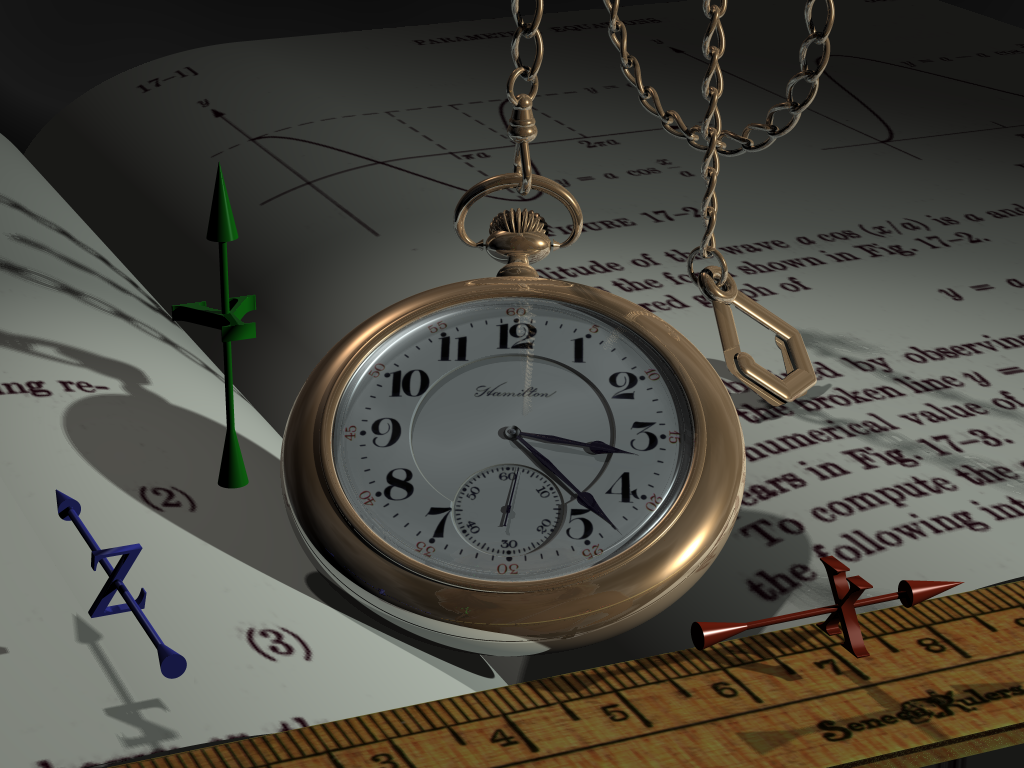
\includegraphics[width=4.4cm]{imagens/watch.png}
    \caption{\texttt{imagens/watch.png}}
    \label{fig:watch}
\end{subfigure}

    \caption{Imagens base da comparação dos filtros.}
    \label{fig:base}
\end{figure}


\end{document}
